\section*{Results}
The following results were found by running experiments on a single desktop computer with an 11th Gen Intel Core i5-11400F 2.60GHz CPU and a Nvidia GeForce GTX 1660 SUPER GPU.

When benchmarking the CuCounter's counter object, we are primarily concerned with the throughput of kmers being counted rather than initialization and lookup. 
Several test runs using a predefined set of 153,627,144 kmers encoded as 64-bit unsigned integers, and encoded kmer data from a synthetic fasta file containing 20 million reads of length 150, yielded a throughput of roughly 1 billion kmers per second.
The throughput is primarily controlled by the underlying hashtable's load factor. The counter also supports taking the reverse complement of each kmer, incrementing the frequency count for these kmers as well. 
Enabling the support for reverse complement counting will roughly halve the throughput.

\begin{figure}[ht!]\label{figure:cucounter_throughput_and_load_factor}
\center
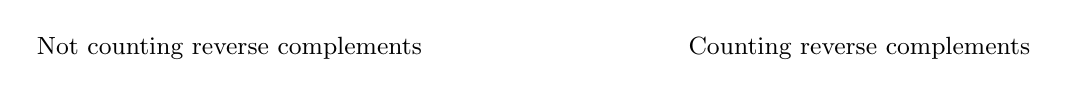
\begin{tikzpicture}[font=\small]
\node at(-4,-0.95)(title){\smaller{Not counting reverse complements}};
\node at(4,-0.95)(title){\smaller{Counting reverse complements}};
\end{tikzpicture}
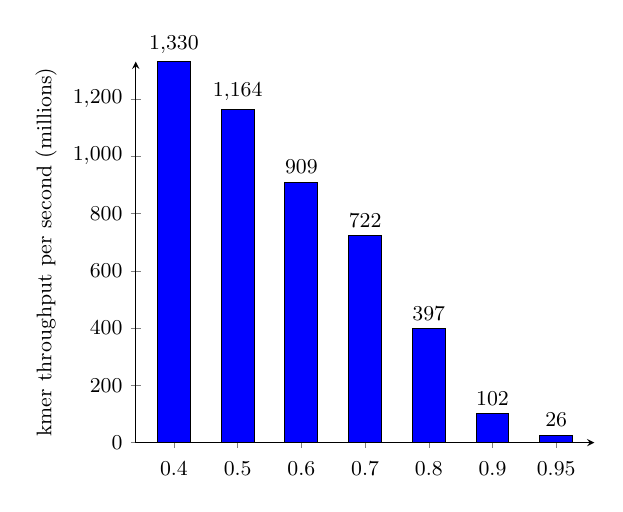
\begin{tikzpicture}[font=\small,scale=0.85]
\begin{axis} [
  ylabel={kmer throughput per second (millions)},
  xlabel={},
  ybar,
  bar width=14pt,
  ymin=0,
  xtick=data,
  axis x line=bottom,
  axis y line=left,
  enlarge x limits=0.1,
  symbolic x coords={0.4,0.5, 0.6, 0.7, 0.8, 0.9, 0.95},
  xticklabel style={anchor=base, yshift=-\baselineskip},
  /pgf/number format/.cd,fixed,precision=3,
  nodes near coords={\small\pgfmathprintnumber{\pgfplotspointmeta}},
  legend style={anchor=west},
]
\addplot[fill=blue] coordinates {
    (0.4, 1330)
    (0.5, 1164)
    (0.6, 909)
    (0.7, 722)
    (0.8, 397)
    (0.9, 102)
    (0.95, 26)
};
\end{axis}
\end{tikzpicture}
\hspace{1.5em}
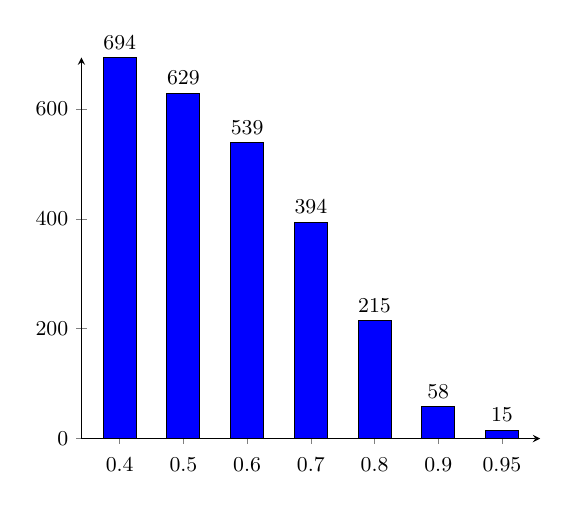
\begin{tikzpicture}[font=\small,scale=0.85]
\begin{axis} [
  ylabel={},
  xlabel={},
  ybar,
  bar width=14pt,
  ymin=0,
  xtick=data,
  axis x line=bottom,
  axis y line=left,
  enlarge x limits=0.1,
  symbolic x coords={0.4,0.5, 0.6, 0.7, 0.8, 0.9, 0.95},
  xticklabel style={anchor=base, yshift=-\baselineskip},
  /pgf/number format/.cd,fixed,precision=3,
  nodes near coords={\small\pgfmathprintnumber{\pgfplotspointmeta}},
  legend style={anchor=west},
]
\addplot[fill=blue] coordinates {
    (0.4, 694)
    (0.5, 629)
    (0.6, 539)
    (0.7, 394)
    (0.8, 215)
    (0.9, 58)
    (0.95, 15)
};
\end{axis}
\end{tikzpicture}

\hspace{3em}
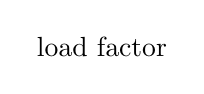
\begin{tikzpicture}[]
\node at(0,0)(xlabel){\smaller{load factor}};
\end{tikzpicture}
\caption{CuCounter kmer throughput per second (in millions) given the underlying hashtable's load factor. Left shows kmer throughput when not counting each kmer's reverse complement, while the right shows the throughput when counting each kmer's reverse complement.}
\end{figure}

CuStats will contain statistical functions useful for graph and alignment-free genotyping. 
Currently only two variants of a single function is are supported. 
The currently supported function is logpmf (log of the probability mass function). 
Both variants of the function have been benchmarked against equivalent NumPy implementations for various input array sizes to demonstrate the dramatic speed increase of performing these array-operations on the GPU. 
For sufficiently large arrays, CuStats achieves up to 120X speed increase over NumPy.

